\documentclass{beamer}
\usetheme{CambridgeUS}
\usecolortheme{beaver}
\usepackage[utf8]{inputenc} 
\title{Rozpoznawanie obrazów}
\author{Paweł Kumorowski}
\date{\today}
\usepackage{amsfonts}
\usepackage[MeX]{polski}
\usepackage{graphicx}
\begin{document}
\frame{\titlepage}


\begin{frame}
\frametitle{Spis Treści}
\tableofcontents
\end{frame}


\section{Wstęp}
\begin{frame}{Rozpoznawanie obrazów}

\begin{figure}
	\centering
		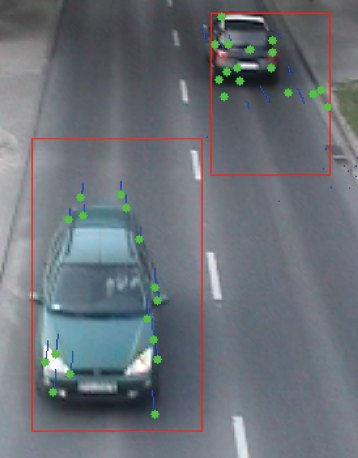
\includegraphics[width=0.2\textwidth]{samochod.jpg}
		\caption{System rozpoznający obiekty}
\end{figure}

\begin{itemize}
\item Rozpoznawanie obrazu --- przetwarzanie obrazu przez maszynę za pomocą urządzeń zewnętrznych w opis cyfrowy tegoż obrazu w celu dalszego przetwarzania.
\end{itemize}
\end{frame}


\section{Wymagania}
\begin{frame}{Wymagania}
\begin{itemize}
\item Do poprawnego rozpoznania tego co znajduje się na obrazie wymagana jest wstępna ,,wiedza''. Człowiek wiedzę potrzebną mu do poprawnego rozpoznawania i~rozumienia istoty rzeczy zbiera bezwiednie poprzez całe swoje życie, maszynę zaś trzeba tej wiedzy "nauczyć".
\pause
\item Sam proces uczenia maszyny może polegać na utworzeniu odpowiedniej bazy danych zawierającej niezbędne reguły i~opis cech przedmiotu.
\end{itemize}
\end{frame}


\section{Prawdziwy cel}
\begin{frame}{Prawdziwy cel}
\begin{itemize}
\item W rozpoznawaniu obrazów bazującym na statystyce naszym celem jest oszacowanie prawdopodobieństwa, czy obiekt, któremu ,,się przyglądamy'' jest tym czy innym obiektem którego opis znajduje się wśród wiedzy posiadanej przez nasz system. 
\pause
\item Dążymy do osiągnięcia 100\% pewności co do zaklasyfikowania obiektu, jednakże tej 100\% pewności nigdy nie osiągamy.
\end{itemize}
\end{frame}


\section{Błąd klasyfikacji}
\begin{frame}{Błąd klasyfikacji}
\begin{itemize}
\item Zadaniem twórcy systemu rozpoznawania obrazu jest skonstruowanie algorytmu, który będzie minimalizował błąd klasyfikacji.
\pause
\item Zakłada się minimalizacje błędu klasyfikacji, a~nie całkowite jego wyeliminowanie.
\pause
\item W prawdziwym świecie, świecie nie cyfrowym, brakuje odpowiedniej wiedzy o~rozkładzie prawdopodobieństwa cech i~klas, i~jedynie cząstkowe informacje są dostępne, w~związku z~tym nie sposób jest całkowicie uniknąć błędu.
\end{itemize}
\end{frame}


\section{Ograniczenia narzucane systemowi}
\begin{frame}{Ograniczenia narzucane systemowi}
Często, aby usprawnić oraz uprościć działanie systemu rozpoznawania obrazów wprowadza się pewne ograniczenia.
\pause
\begin{itemize}
\item Pytania zadawane systemowi sprawdzają się do sformowania jaki obiekt najprawdopodobniej występuje na obrazie.
\pause
\item Odpowiedzią jest obiekt klasy która w drodze ewaluacji dostał najwyższą notę prawdopodobieństwa.
\pause
\item Zestaw danych opisujących obiekt przeznaczony do rozpoznania ograniczone są do skończonego zestawu cech.
\end{itemize}
\end{frame}


\section{Klasyfikacja obiektów}
\begin{frame}{Klasyfikacja obiektów in. rozpoznawanie wzorców}
Istnieją dwa ogólne podejścia do klasyfikacji obrazów, które to dzieli się na pomniejsze, konkretyzujące sposób rozwiązywania tego problemu.
\pause
\begin{itemize}
\item Podejście pierwsze: decyzyjno-teoretyczne (ang. decision-theoretical)\
\pause
\item Podejście drugie: strukturalne (składniowe, lingwistyczne)
\end{itemize}
\end{frame}


\begin{frame}{Podejście pierwsze: decyzyjno-teoretyczne}
\begin{itemize}
\item W tym podejściu zakładamy, że nasz wzór/obiekt jest reprezentowany poprzez wektor liczb zwanych wartościami cech. 
\pause
\item Cechy te możemy wyznaczyć samemu na podstawie wstępnej analizy obiektu, która ma na celu wyłonienie istotnych cech, bądź mogą być ona nam narzucone z góry.
\end{itemize}
\end{frame}


\begin{frame}{Podejście drugie: strukturalne}
\begin{itemize}
\item W tym przypadku obiekt, tj. wzorzec, opisywany jest za pomocą ogromnej, ale skończonej ilości pod-wzorców/bazowych elementów oraz ,,gramatykę'', która określa w jaki sposób pod-wzorce/bazowe elementy budują obiekt.
\pause
\item W tym podejściu problem rozpoznania obiektu na obrazie sprowadzony jest więc do odpowiedzi na pytanie: czy dany wzór przynależy do języka tworzonego przez zdefiniowaną przez nas gramatykę?
\end{itemize}
\end{frame}


\section{Uczenie}
\begin{frame}{Uczenie}
\begin{itemize}
\item Uczenie jest sposobem pozyskiwania wiedzy przez system i jest niezbędnym etapem przygotowującym system do rozpoznawania obiektów.
\end{itemize}
\end{frame}


\begin{frame}{Przygotowanie materiałów uczących}
Dane za pomocą których będziemy uczyć system rozpoznawania obiektów wybranej kategorii/klasy poddawane są wstępnej obróbce mającej na celu uproszczenie obrazu do tego stopnia aby zawierał jedynie minimalną ilość danych niezbędnych do rozpoznania obiektu.
\pause
\begin{itemize}
\item Dane obrazowe
\pause
\item Dane nieobrazowe --- Szkieletyzacja 
\end{itemize}
\end{frame}


\begin{frame}{Szkieletyzacja (ang. skeletonization)}
\begin{itemize}
\item Jest to proces, który umożliwia uzyskanie szkieletu obiektu czyli jego punktów osiowych.
\pause
\item Przez szkielet rozumiemy zbiór wszystkich możliwych środków maksymalnych okręgów, które można wpisać w środek obiektu.
\pause
\item W wyniku operacji szkieletyzacji cały obiekt zostaje zredukowany do zbioru linii o szerokości jednego punktu.
\pause
\end{itemize}

\begin{figure}
	\centering
		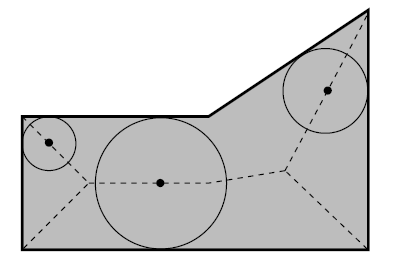
\includegraphics[width=0.2\textwidth]{szkieletyzacja.png}
		\caption{Przykładowy kształt oraz jego szkielet}
\end{figure}

\end{frame}


\end{document}
